\documentclass{beamer}

\usetheme{Antibes}

\usepackage[ngerman]{babel}
\usepackage[utf8x]{inputenc}
\usepackage{totpages}
\usepackage{graphicx}
\usepackage[export]{adjustbox}
\usepackage{multicol}
\usepackage{listings} 
\lstset{ 
    language=html, 
    basicstyle=\ttfamily, 
    keywordstyle=\color{blue}, 
} 
\usepackage{xcolor}

\setbeamercovered{transparent}
\beamertemplatenavigationsymbolsempty
%\setbeamertemplate{footline}[frame number]
\setbeamertemplate{footline}
  {%
    \begin{beamercolorbox}[ht=2.5ex,dp=1.125ex,%
      leftskip=.3cm,rightskip=.3cm plus1fil]{upper separation line foot}
       \hfill Folie~\thepage / \ref{TotPages}
    \end{beamercolorbox}
    \begin{beamercolorbox}[ht=2.5ex,dp=1.125ex,%
      leftskip=.3cm,rightskip=.3cm plus1fil]{author in head/foot}%
      \leavevmode{\usebeamerfont{author in head/foot}\insertshortauthor}%
      \hfill%
      {\usebeamerfont{institute in head/foot}\usebeamercolor[fg]{institute in 						head/foot}\insertshortinstitute}%
    \end{beamercolorbox}%
    \begin{beamercolorbox}[colsep=1.5pt]{lower separation line foot}	
    \end{beamercolorbox}
  }
  
\title{ChromecastV2 - Google Cast API}
\author{N. Vetter}
\date{\today}

\institute[Universität Potsdam]{
	Institut für Informatik
}

\begin{document}

\begin{frame}

\titlepage

\end{frame}

\section{Allgemeines}
\subsection{Vorstellung}
\begin{frame}

\begin{itemize}
\item finden der Empfänger durch mDNS und UPNP
\item aufgeteilt in Sender und Empfänger API
\item Sender API verfügbar für Android, Chrome, iOS
\item Standard und Custom Empfänger möglich
\item Verteilung der Empfänger-Applikation zwingend über HTTPS 
\item zentraler Suchdienst für Apps (Google Datenbank)
\item hauptsächlich Nachrichtenbasierte Kommunikation
\end{itemize}
\end{frame}

\section{Übersicht}
\begin{frame}
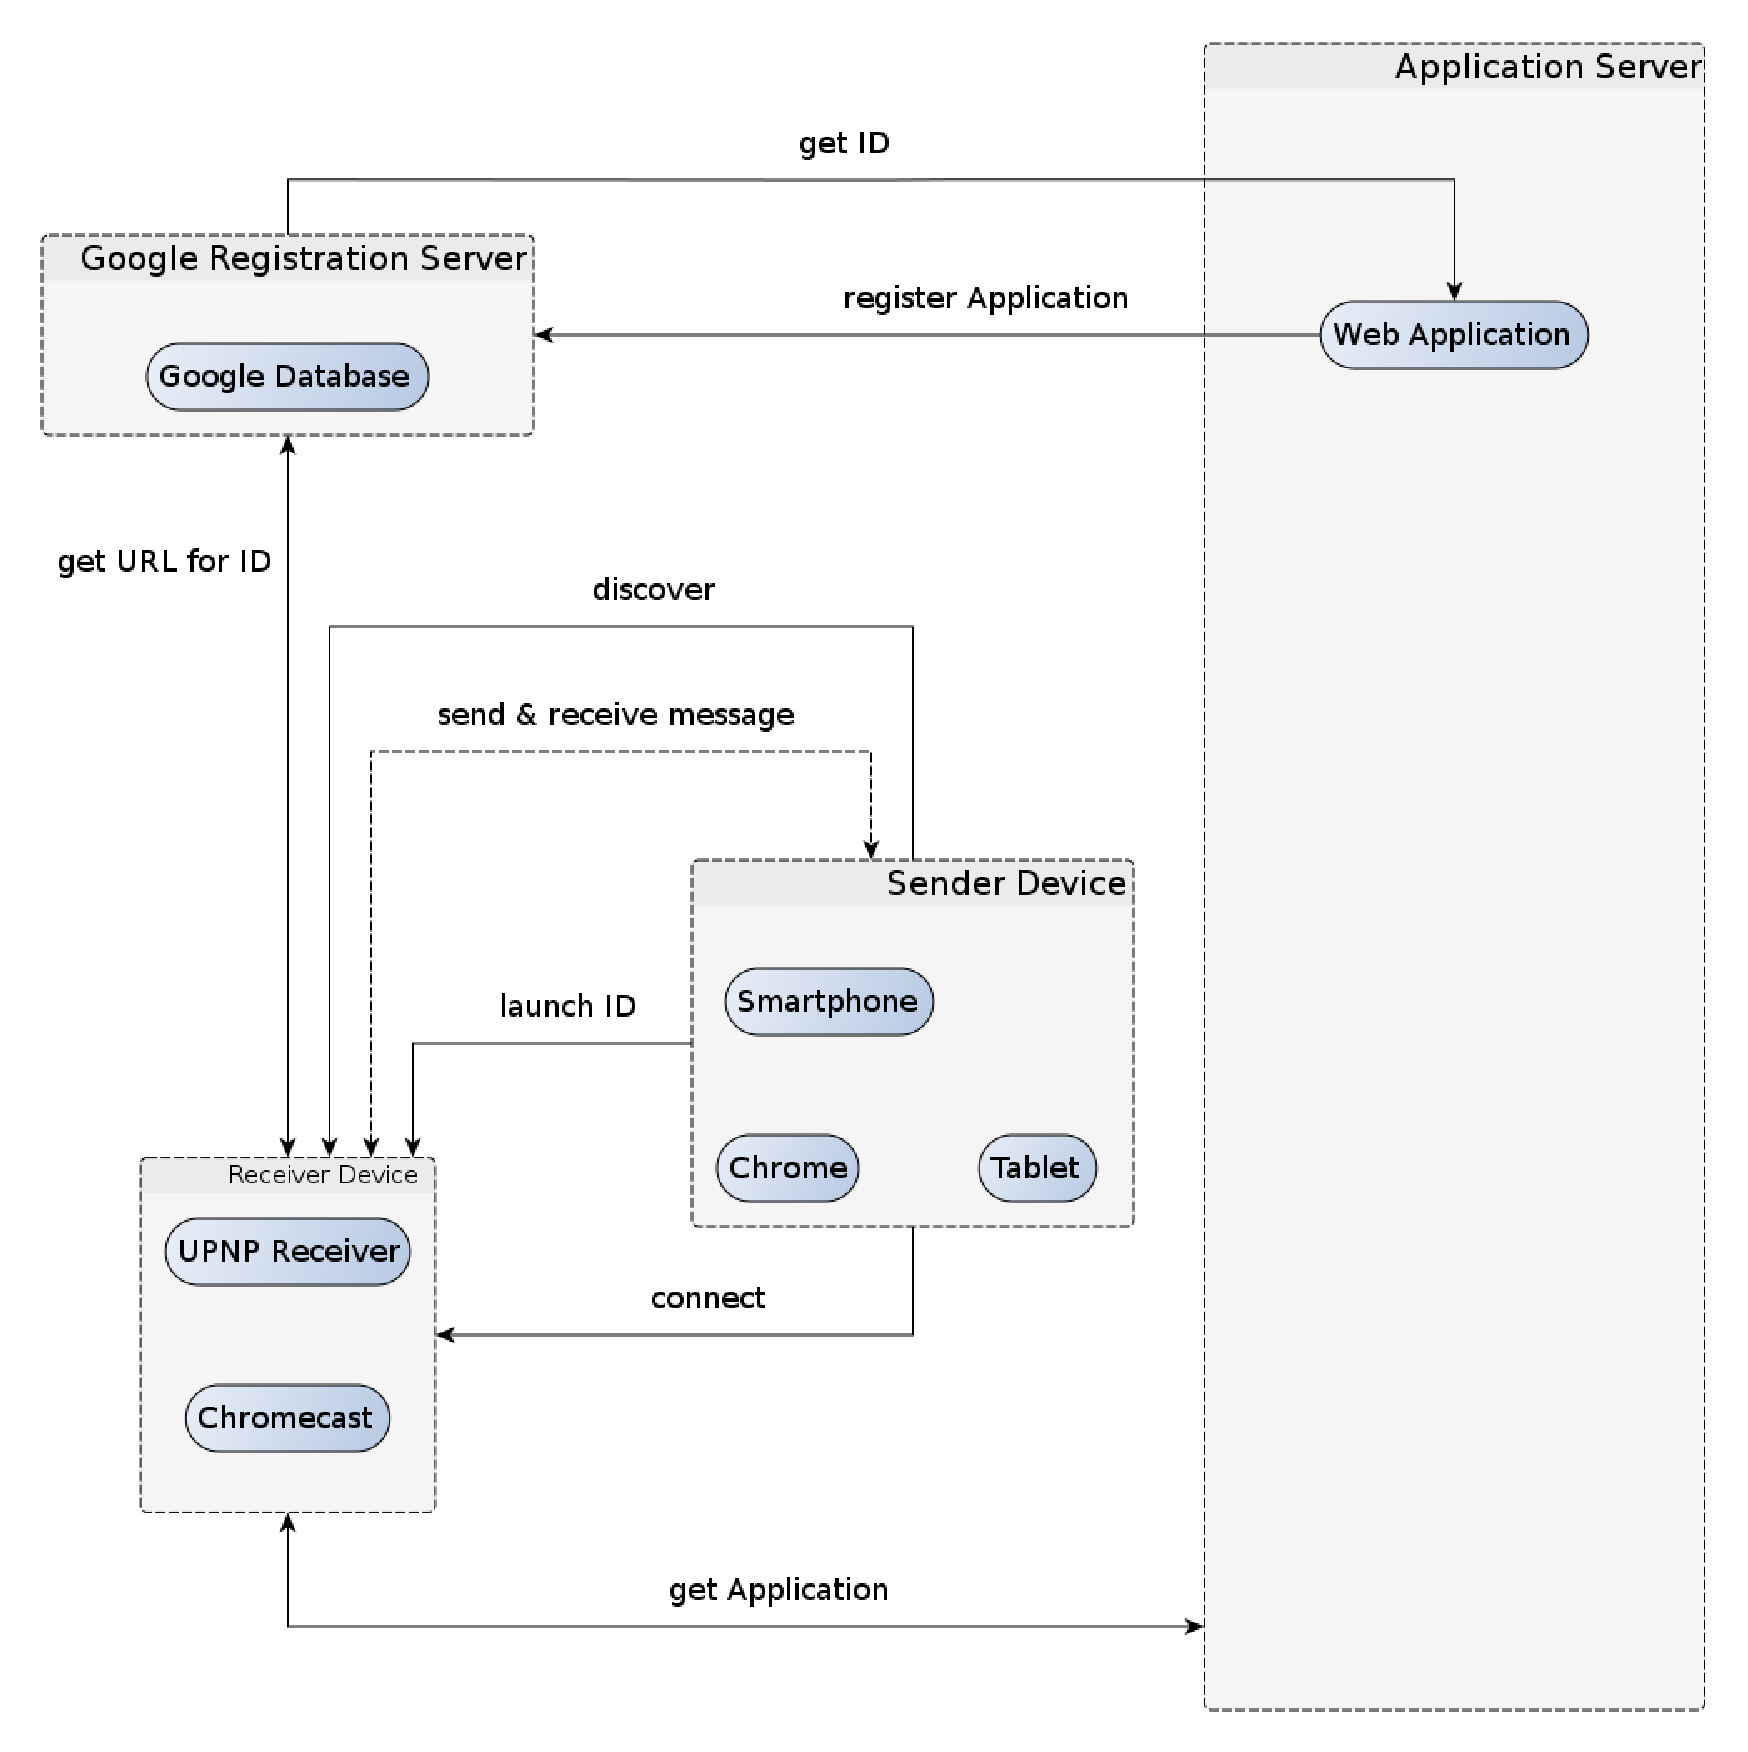
\includegraphics[scale=0.28]{neu0.eps}
\end{frame}

\section{Beispiel}


\begin{lstlisting}[basicstyle=\tiny]
<html>
<head>
  <title>Example minimum receiver</title>
  <script src="//www.gstatic.com/cast/sdk/libs/
  				receiver/2.0.0/cast_receiver.js"></script>
</head>
<body>
  <video id='media'/>
  <script>
    window.mediaElement = document.getElementById('media');
    window.mediaManager = new cast.receiver.MediaManager(window.mediaElement);
    window.castReceiverManager = cast.receiver.CastReceiverManager.getInstance();
    window.castReceiverManager.start();
  </script>
</body>
</html>
\end{lstlisting}
\end{document}